\documentclass[a4paper,12pt]{article}
\usepackage{fullpage}
\usepackage{setspace}
\usepackage[utf8]{inputenc}
\usepackage[T1]{fontenc}
\usepackage[french]{babel}
\usepackage{enumitem}
\usepackage[final]{pdfpages}
\usepackage{graphicx}
\usepackage{pgfgantt}
\usepackage[colorlinks=true,linkcolor=black,urlcolor=black]{hyperref}
\usepackage{microtype}
\usepackage{color}
\usepackage{listings}
\frenchbsetup{StandardLists=true}
\DisableLigatures[<,>]{encoding=T1,family=tt*}
\setitemize[0]{label=$-$}
\begin{document}
% PAGE DE GARDE
	\begin{flushright}
		
\includegraphics[scale=0.3]{UGA.eps}
	\end{flushright}
	\vspace{1.5cm}
	\begin{center}
		{\Large Universit\'e{} Joseph Fourier\\
		D\'e{}partement Licence Sciences \& Technologie}\\
		\vspace{1cm}
		{\Huge RAPPORT DE STAGE}\\
		\vspace{3mm}
		{\Large Calcul parall\`ele sur GPU}\\
		\vspace{2mm}
		Picard Micha\"el\\
		6 juin 2016 - 1er juillet 2016\\
		\vspace{4mm}
		\includegraphics[scale=0.3]{LIG.eps}
		\includegraphics[scale=0.3]{INRIA.eps}
	\end{center}
	\vspace{1cm}
	\begin{flushleft}
		Laboratoire d'accueil : LIG - INRIA\\
		\'E{}quipe : POLARIS\\
		Directeur du laboratoire : GAUSSIER Eric (LIG)\\
		\hspace{4.65cm} GROS Patrick (INRIA)\\
		Responsable du stage : HUARD Guillaume
	\end{flushleft}
	\vspace{8mm}
	\begin{flushright}
	License MIN - 1\`ere ann\'e{}e\\
	Ann\'e{}e universitaire : 2015 - 2016
	\end{flushright}
	
	\newpage
	{\scriptsize Cette page a \'e{}t\'e{} laiss\'e{} intentionnellement blanche.
	\newpage
%SOMMAIRE
	\renewcommand{\contentsname}{
		\begin{center}
			Sommaire
		\end{center}
	}
	\setcounter{tocdepth}{3}
	\tableofcontents
% CORPS DU RAPPORTS
	\newpage
	\section{Remerciement}
		\indent Je tiens à remercier Mr HUARD Guillaume pour son accueil au sein de l'équipe Polaris, pour sa gentillesse et pour le temps qu'il m'a accord\'e{} pour m'expliquer de nouvelles notions, tant utilitaire, m\'e{}thodique qu'algorithmique, pour ses encouragements et son soutien durant ce stage, qui m'a permis de d\'e{}couvrir le m\'e{}tier d'enseignant-chercheur. \\
		\indent Je remercie aussi Mr BENIAMINE David, actuellement en th\`ese à l'INRIA, pour le temps pass\'e{} à m’accueillir sur les locaux et ses conseils utiles pour me permettre d'avancer durant le stage.\\
		\indent Je remercie Mme SIMON Annie, l'assistante de l'\'e{}quipe Polaris pour son temps sur mon dossier, et pour m'avoir aid\'e{} à r\'e{}gler les nombreux impr\'e{}vus à propos des conventions de stage et autres formalit\'e{}s.\\
		\indent Je remercie aussi l'INRIA et le LIG ainsi que leurs directeurs respectifs, Mr GAUSSIER Eric et Mr GROS Patrick, pour m'avoir permis de participer \`a une pr\'e{}sentation d'algorithmie pour des lycéens, dans leurs locaux de Montbonnot, sous la tutelle de Mr HUARD.\\
		\indent Je remercie enfin l'UGA, le DLST et Mmes MANDON Nina, COGNE Lydie, DARRACQ Marie-Cécile et CAJOT Patricia pour m'avoir donné l'opportunité de participé à ce stage.
	\newpage
	\section{Introduction}
	\indent Mon stage à l'Inria portant sur le Calcul parall\`ele sur GPU, j'ai \'e{}t\'e{} amen\'e{} à utiliser de nombreux outils.\\
	\noindent Je vais donc vous pr\'e{}senter en premier lieu la structure d'accueil du stage, puis je vous parlerai des différents outils utilisée durant ce stage, la raison pour laquelle j'ai choisi ce stage, avant de vous pr\'e{}senter mon \'e{}volution durant mes 4 semaines en tant que stagiaire.
	\subsection{Environnement d'acceuil : INRIA \& LIG}
	\indent L’INRIA est un centre de recherche cr\'e{}\'e{} \`a sous le r\'e{}gime du G\'e{}n\'e{}ral De Gaule et compte aujourd’hui presque une dizaine de centres en France. Le centre Rh\^one-Alpes a \'e{}t\'e{} cr\'e{}\'e{} en 1992.\\
	\indent \`A Grenoble le directeur du centre est Mr GROS Patrick depuis le 1er D\'e{}cembre 2014. La plupart des \'e{}quipes-projets INRIA grenobloises sont des \'e{}quipes communes avec le CNRS, l’Universit\'e{} Joseph Fourier (maintenant Universit\'e{} Grenoble Alpes), et Grenoble INP au sein des laboratoires :
    \begin{itemize}
        \item Laboratoire d’Informatique de Grenoble (LIG)
        \item Laboratoire Jean Kuntzmann (LJK)
        \item Laboratoire Grenoble Images Parole Signal Automatique (GIPSA)
        \item Laboratoire Adaptation et Pathog\'e{}nie des Microorganismes (LAPM)
    \end{itemize}
    Le LIG est quant \`a lui compos\'e d'une multitude d'\'e{}quipe :
    \begin{itemize}
        \item POLARIS
        \item DATAMOVE
        \item DRAKKAR
        \item ERODS
        \item ...
    \end{itemize}
	\indent \indent L'\'e{}quipe qui m'a accueilli est l'\'e{}quipe POLARIS, nouvellement install\'e{}e au b\^atiment IMAG sur le campus universitaire de Grenoble. Le responsable du LIG est Mr GAUSSIER Eric, tandis que le responsable de l'\'e{}quipe POLARIS est Mr Legrand Arnaud. Le thème de recherche de cette \'e{}quipe est << Calcul distribu\'e et \`a haute performance~ >>, plus pr\'e{}cis\'e{}ment << Performance analysis and optimization of LARge Infrastructures and Systems >>.
	\subsection{Outils et M\'e{}thodes utilis\'e{}s}
	\indent Dans cette partie, je vais vous pr\'e{}senter les diff\'e{}rentes m\'e{}thodes de travail et les languages (et logiciel) appris pour ce stage.
	\subsubsection{CUDA et les cartes graphiques NVIDIA}
	\indent Tout d'abord, il est n\'e{}cessaire de rappeler le sujet du stage : le calcul parall\`ele, plus pr\'e{}cis\'e{}ment sur GPU. Pour expliquer le choix de ce language, il est n\'e{}cessaire de faire quelque petits rappels. \\
	\indent Le CPU (Central Processing Unit ou processeur) est le c\oe{}ur de l'ordinateur, c'est lui qui ex\'e{}cute toutes les commandes et calculs requis par l'ordinateur. Avec l'\'e{}volution des programmes informatiques, la puissance des c\oe{}urs des processeurs a d\^u augmenter, jusqu'en atteindre une limite physique en 2003, qui induisit la cr\'e{}ation de processeurs multic\oe{}urs pour augmenter les performances de notre mat\'e{}riel informatique. Mais le principal probl\`eme est qu'un programme s\'e{}quentiel ne va s'ex\'e{}cuter que sur un seul coeur d'un processeur multic\oe{}ur, ce qui ne permettait pas d'obtenir de gain de temps (d'ex\'e{}cution) efficace, d'o\`u les d\'e{}buts de la programmation parall\`ele. \\
	\indent Dans le m\^eme temps, les cartes graphiques ou GPU (qui sont accessible au grand public depuis 1981) ont \'e{}t\'e{} d\'e{}velopp\'e{} : principalement utilis\'e{}es pour le rendu d'image en 2D/3D, il a \'e{}t\'e{} rapidement d\'e{}couvert que, gr\^ace \`a leur structure si particuli\`ere (elles poss\`edent un grand nombre de c\oe{}urs de calcul simple au d\'e{}triment de la complexit\'e{} des instructions et de la m\'e{}moire fourni), il est possible d'ex\'e{}cuter de multiples calculs simultan\'e{}ment, gagnant un temps de calculs d\'e{}pendant de la taille des donn\'e{}es (plus il y a de donn\'e{}es, plus le gain est important) si l'on compare à un c\oe{}ur de CPU. Donc, les principales entreprises de production de cartes graphiques (NVidia et AMD) ont d\'e{}vellop\'e{} leur propre language de programmation parall\`ele, adapt\'e{} des languages de programmation existants, tel que le C et le C++ (il s'ag\^it d'extension des languages).
	\medbreak
	\indent Pour en revenir avec le sujet du stage, nous allons donc faire du calcul parall\`ele et ce, sur le GPU. \'E{}tant donn\'e que les cartes graphiques du laboratoire sont des cartes graphiques NVidia, il a \'e{}t\'e choisi d'utiliser le language CUDA, d\'e{}velopp\'e par NVidia exclusivement pour leur produit. \`A noter qu'il aurait tout aussi bien pu \^etre possible d'utiliser un autre language.
	\\ \indent Pour bien utiliser et comprendre CUDA (\`a partir de maintenant, CUDA sera consid\'e{}r\'e{}e comme une extension du C, car nous avons travaill\'e{} avec celle originaire du C, mais il existe des versions C++,Python,...), il me parait n\'e{}cessaire de comprendre comment est form\'e{}e une carte graphique.
	\begin{figure}
	    \centering
	    \caption{Structure d'un GPU}
	    \label{fig:structGPU}
	    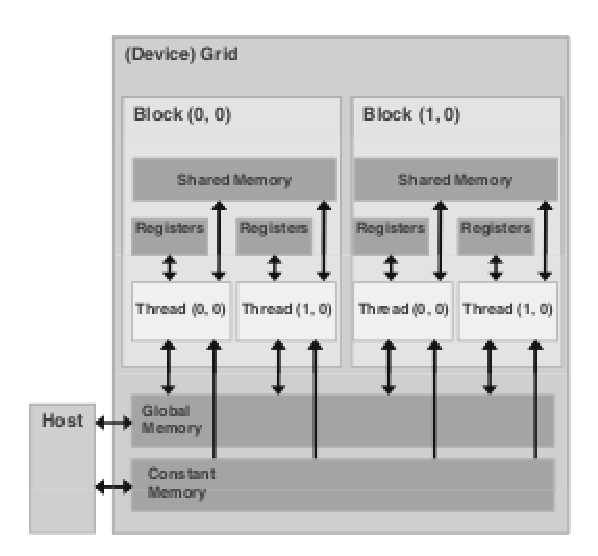
\includegraphics[scale=0.65]{Shema_structure_GPU.eps}
	\end{figure}
    Dans la figure~\ref{fig:structGPU} est décrite la structure d'un GPU, la carte graphique \'e{}tant compos\'e{}e :
    \begin{itemize}
        \item d'une grille (Grid) qui comprend tout les \'e{}l\'e{}ments du GPU ;
        \item de 2 DRAM (Dynamic Random Access Memory), qui stockent les donn\'e{}es modifiables pour l'une et les constantes pour l'autre, accessible par l'h\^ote (i.e. le CPU, et seulement par transfert) et par tous les autres composants du GPU ;
        \item de multiples Blocks (en quantit\'e{} d\'e{}pendante du GPU) qui rassemble :
        \begin{itemize}[label=$+$]
            \item une m\'e{}moire cache (Shared Memory) et une m\'e{}moire texture (non affich\'e{}e sur le sch\'e{}ma, de tr\`es faible capacit\`e{}e et principalement pour les graphiques) accessible par tous les composants du Block ;
            \item de multiples c\oe{}urs de calculs (Thread, en quantit\'e{}s d\'e{}pendants du GPU) de calculs ;
            \item de 2 m\'e{}moires locales (Registered et Local) propres \`a chaque Thread qui permet le stockage de tableaux de donn\'e{}es dans la m\`emoire Local et d'autres donn\'e{}es dans la m\'e{}moire Registered.
        \end{itemize}
    \end{itemize}
    De plus, le GPU ne peut pas acc\'e{}der \`a des donn\'e{}es stock\'e{}es sur les disque durs, la RAM et les m\'e{}moires internes du CPU, tandis que le CPU ne peux que faire des \'e{}changes de donn\'e{}es entre la RAM (de lui-m\^eme) et la DRAM (du GPU). \\
    D'o\`u l'introduction de nouvelles fonctions, li\'e{}es au concept de la parall\`elisation des calculs :
    \begin{itemize}
        \item l'\'e{}quivalent du \textcolor{blue}{malloc()} et du \textcolor{blue}{free} sont \textcolor{green}{cudaMalloc} et \textcolor{green}{cudaFree}, pour allouer sur la Global Memory ;
        \item pour effectuer des calculs sur le GPU, il est n\'e{}cessaire de cr\'e{}er des fonctions r\'e{}pondant \`a la norme : \textit{parametre type fonction(variable)} o\`u le param\`etre est un identifiant que indique si l'appel se fait du CPU vers le GPU (~\textit{\_\_global\_\_}~) ou du GPU vers le GPU (~\textit{\_\_device\_\_}~), de type au choix sauf si le parametre \_\_global\_\_ est d\'e{}fini et le type \textit{void} est alors obligatoire. L'appel de cette m\^eme fonction se fait de la forme \textit{fonction<{}<{}<dimGrid,dimBlock>{}>{}>(variable)}, o\`u dimGrid et dimBlock sont les dimensions de la grille et de chaque block, que l'on défini et limit\'e \`a une dimension d\'e{}pendant de la carte graphique ;
        \item dans le corps d'une fonction du GPU, chaque thread executera sa propre version de la fonction, et toute variable interne \`a la fonction sera propre \`a chaque thread (sauf si elle est d\'e{}clar\'e{}e \textit{\_\_shared\_\_}) si qui implique que l'on peux avoir \`a faire appel \`a des variables tels que threadIdx.x (ou .y/.z) pour connaitre l'emplacement du thread dans son block (voir figure~\ref{fig:structGrid} pour un exemple) ;
        \item la compilation se fait avec nvcc (il est possible que la compilation est des erreurs sans r\'e{}ponses, pour les corriger [si il ne s'agit pas d'erreur de votre part] il suffit de renommer vos fichiers *.c en *.cpp car le compilateur nvcc est plus adapt\'e au C++ qu'au C).
    \end{itemize}
	\begin{figure}
	    \centering
	    \caption{Exemple d'une grille d\'e{}fini par une fonction}
	    \label{fig:structGrid}
	    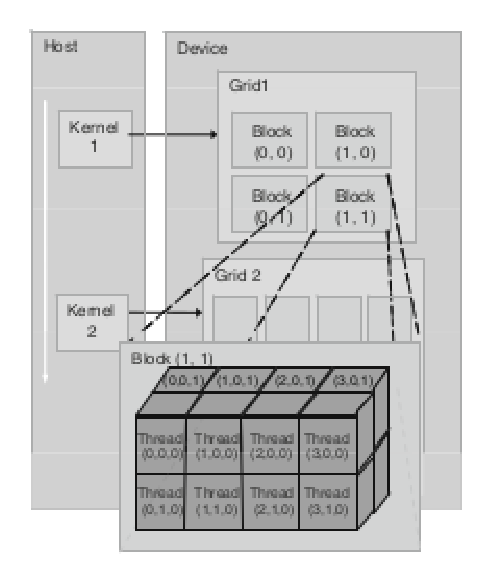
\includegraphics[scale=0.65]{Structure_grille_GPU.eps}
	\end{figure}
	\subsubsection{GIT}
	\indent Selon \url{https://git-scm.com/book/fr/v1/D%C3%A9marrage-rapide-Une-rapide-histoire-de-Git} :
	\\ \textit{Comme de nombreuses choses extraordinaires de la vie, Git est n\'e avec une dose de destruction cr\'e{}ative et de controverse houleuse. Le noyau Linux est un projet libre de grande envergure. Pour la plus grande partie de sa vie (1991–2002), les modifications \'e{}taient transmises sous forme de patchs et d'archives de fichiers. En 2002, le projet du noyau Linux commen\c{c}a \`a utiliser un DVCS propri\'e{}taire appel\'e BitKeeper. \\
En 2005, les relations entre la communaut\'e d\'e{}veloppant le noyau Linux et la soci\'e{}t\'e en charge du d\'e{}veloppement de BitKeeper furent rompues, et le statut de gratuit\'e{} de l'outil fut r\'e{}voqu\'e. Cela poussa la communaut\'e du d\'e{}veloppement de Linux (et plus particuli\`erement Linus Torvalds, le cr\'e{}ateur de Linux) \`a d\'e{}velopper son propre outil en se basant sur les le\c{c}ons apprises lors de l'utilisation de BitKeeper. Certains des objectifs du nouveau syst\`eme \'e{}taient les suivants :
\begin{itemize}[parsep=0cm,itemsep=0cm,topsep=0cm]
    \item vitesse ;
    \item conception simple ;
    \item support pour les d\'e{}veloppements non lin\'e{}aires (milliers de branches parall\`eles) ;
    \item compl\`etement distribu\'e ;
    \item capacit\'e à g\'e{}rer efficacement des projets d'envergure tels que le noyau Linux (vitesse et compacit\'e des donn\'e{}es).
\end{itemize}
}
	\begin{figure}[!h]
	    \centering
	    \caption{Fonctionnement de GIT}
	    \label{fig:funcGIT}
	    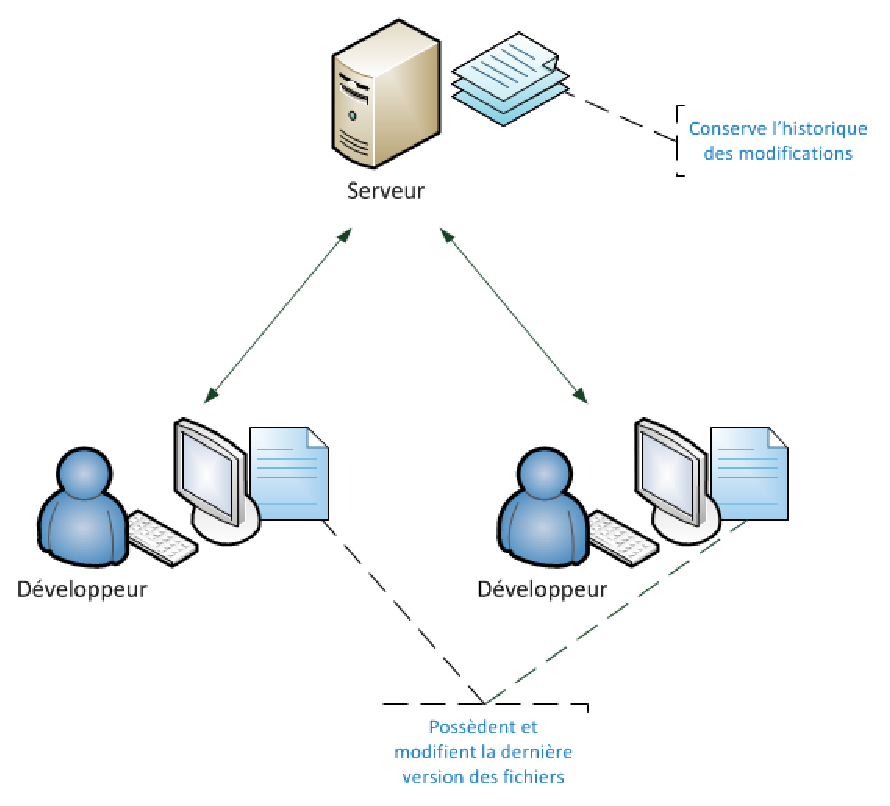
\includegraphics[scale=0.65]{shema_git.eps}
	\end{figure}
	\indent Ainsi, GIT est plus un gestionnaire de version en ligne, centralis\'e pour permettre un acc\`es depuis plusieurs appareils. Ce service fonctionne sous le principe suivant (voir figure \ref{fig:funcGIT}) : un serveur possède chaque version du projet, et permet \`a chaque client de poss\'e{}der une version commune \`a tous du projet, qu'il modifiera de manière locale avant de la retransmettre au serveur, en prenant garde de r\'e{}gler tout conflit qui pourrait lui \^etre signaler (d\^u \`a la mise \`a jour du projet par un autre client avant vous), ce qui permet d'avoir un suivi complet du projet par tous les d\'e{}veloppeur (client) de pouvoir travailler en collaboration sans problème de gestion. \`A noter qu'il est possible de multiplier ou diviser les branches de d\'e{}veloppement, pour permettre de partir dans plusieurs direction de recherche sans compromettre le travail ex\'e{}cuter pr\'e{}c\'e{}demment. Ce qui en fait un des gestionnaire de version les plus puissants existants.\\
	De fait, il existe des d\'e{}p\^ots en ligne tel que GitHub.com qui permettent d'obtenir gratuitement un "serveur" pour centraliser ses donn\'e{}es gratuitement (mais les donn\'e{]es sont accessibles et non modifiables par tous) ou en payant pour un "serveur" privé.
	Par exemple, ceci est mon GIT pour ce stage : \url{https://github.com/mipicard/Stage_parrallel_programming}
	\subsubsection{Abstraction et factorisation du code}
	\indent Ici, nous allons expliquer quelques m\'e{}thodes de travail n\'e{}cessaire en laboratoire (surement aussi en entreprise) de programmation :
	\begin{itemize}
		\item \textbf{l'abstraction} : lorsque l'on cr\'e{}\'e un projet, il est plus utile de cr\'e{}e ses propres types (en renommant un type existant ou en construisant le sien) car il est ainsi possible de changer les composants de ce type sans devoir changer tout ce qui utilise ce type et ses fonctions (sauf possiblement les fonctions d\'e{}di\'e{}es ce type, bien entendu) ce qui permet de mettre \`a jour bien plus facilement ses projets sans devoir changer tout son code. De plus, il est utile de s\'e{}parer son code en de multiple petit fichier, par exemple en cr\'e{}ant un fichier pour chaque type, ou par action : le choix est \`a la discr\'e{}tion du d\'e{}veloppeur.
		\item \textbf{la factorisation} : il s'agit d'un effet \`a \'e{}viter lors du d\'e{}veloppement qui consiste a r\'e{}p\'e{}ter inutilement des parties de codes. Il est donc n\'e{}cessaire de rester attentif lorsque l'on code, et si l'on r\'e{}p\`ete du code, de v\'e{}rifier que si c'est obligatoire (autre type) ou si l'on pourrait faire mieux sans r\'e{}p\'e{}tition.
	\end{itemize}
	\subsubsection{R et Rmarkdown}
	\indent Selon \url{https://fr.wikipedia.org/wiki/R_(langage_de_programmation_et_environnement_statistique)} :\\
	\textit{R est un logiciel libre de traitement des donn\'e{}es et d'analyse statistiques mettant en \oe{}uvre le langage de programmation S. C'est un projet GNU fond\'e sur l'environnement d\'e{}velopp\'e dans les laboratoires Bell par John Chambers et ses coll\`egues. Depuis plusieurs ann\'e{}es, deux nouvelles versions apparaissent au printemps et à l'automne. Il dispose de nombreuses fonctions graphiques.\\
Le logiciel R est consid\'e{}r\'e par ses cr\'e{}ateurs comme \'e{}tant une ex\'e{}cution de S, avec la s\'e{}mantique d\'e{}riv\'e{}e du langage Scheme. C'est un logiciel libre distribu\'e{} selon les termes de la licence GNU GPL et disponible sous GNU/Linux, FreeBSD, NetBSD, OpenBSD, Mac OS X et Windows.\\
Une enqu\^ete men\'e{}e par Rexer Analytics aupr\`es de 1 300 analystes retrouve que R est le logiciel le plus souvent utilis\'e{} lorsqu'il s'agit d'un travail en entreprise, dans le monde acad\'e{}mique, au sein d'organismes publics ou d'ONG et chez les analystes travaillant comme consultants.}\\
    \indent R est ainsi un language tr\`es utilis\'e par les chercheurs en informatique pour leur permettre d'obtenir de mani\`ere rapide et optimis\'e{}e des courbes et des r\'e{}sultats leur permettant de r\'e{}pondre \`a leur sujet de recherche. \\
    R est tr\`es souvent utilis\'e en Rmarkdown, i.e en script convertible en page web ou pdf, pour permettre de rassembler de manière efficace le sujet et les r\'e{}sultats d'exp\'e{}riences (voir figure \ref{fig:rmd} pour un exemple tir\'e{} de mon propre fichier rmd).~
	\begin{figure}[!ht]
	    \centering
	    \caption{Exemple de code Rmarkdown}
	    \label{fig:rmd}
	    \includegraphics[scale=0.3]{RMD.eps}
	\end{figure}
	\subsubsection{\LaTeX}
	\indent Selon \url{http://www.grappa.univ-lille3.fr/FAQ-LaTeX/1.1.html} :\\ \textit{TeX (1978) est le formateur de texte de D. E. Knuth. \`A l'origine, Knuth a développé TeX notamment pour réaliser de beaux documents et \'e{}crire des formules mathématiques.\\
    LaTeX, écrit par L. Lamport (1982), est un jeu de macros au-dessus de TeX, plus facile à utiliser que ce dernier. Il
propose notamment différents styles de document auxquels
correspondent des classes de document et une grande diversité
de macros qui répondent à divers besoins des auteurs. LaTeX a
été conçu pour rédiger des articles, des rapports, des thèses ou
des livres ou pour préparer des transparents. On peut insérer
dans le texte, des dessins, des tableaux, des formules
mathématiques et des images sans avoir à se soucier (ou presque)
de leur mise en page. Les documents produits avec LaTeX et TeX
sont d'une excellente qualité typographique.} \\
\indent \LaTeX est donc utilis\'e pour de la mise en forme de texte : il se diff\'erencie de OpenOffice et Microsoft Word par sa compilation, qui permet un meilleur rendu (puisque l'utilisation d'algorithme de traitement plus lourd et efficace) que les autres (qui utilise des algorithmes l\'e{}ger pour un rendu graphique en temps r\'e{}el). Ainsi, il est n\'e{}cessaire d'\'e{}crire dans le texte les sp\'e{}cification graphique comme l'inclusion d'image, la taille, la couleur et le style du texte, etc (voir figure \ref{fig:Latex} pour un exemple tir\'e{}e de notre fichier pour obtenir ce rapport).~
	\begin{figure}[!ht]
	    \centering
	    \caption{Exemple de code \LaTeX}
	    \label{fig:Latex}
	    \includegraphics[scale=0.3]{Latex.eps}
	\end{figure}
	\subsection{Pourquoi ce stage?}
	\indent J'ai choisi ce stage en regardant r\'e{}gulièrement sur le site du DLST, o\`u j'avais remarqu\'e ce stage propos\'e pour l'ann\'e{}e derni\`ere et qui m'avait tr\`es int\'e{}ress\'e : \'e{}tant un grand joueur sur PC, je poss\`ede et j'exploite ma carte graphique pour les jeux et je voulais savoir ce que je pouvais faire d'autre avec, ainsi que l'id\'e{}e de pouvoir r\'e{}ellement faire des ex\'e{}cutions parall\`eles au lieu de toujours le simul\'e en encha\^inant tr\`es rapidement des instructions sens\'e{}es \^etre parall\`eles.
	\newpage
	\section{Mon parcours}
	\indent Le but de ce stage \'e{}tait de d\'e{}couvrir la programmation parall\`eles sur GPU, en utilisant CUDA pour les cartes graphiques NVidia. Pour ce faire, nous avons utilis\'e l'exemple de la multiplication matricielle, qui permet de montrer efficacement les diff\'e{}rences de vitesse d'ex\'e{}cution entre des algos parall\`elis\'e{}s ou non.
	\subsection{L'avancement chronologique}
	\indent Durant la premi\`ere semaine de stage, nous avons d\^u suivre le programme de ce livre \href{http://www.hds.bme.hu/~fhegedus/C++/programming_massively_parallel_processors.pdf}\textit{Programming massively parallel processors}} (disponible ici \url{http://www.hds.bme.hu/~fhegedus/C++/programming_massively_parallel_processors.pdf}) . Ainsi, nous avons suivi le tutoriel en apprenant le language et les exemples, qui seront aussi nos algorithmes de calcul durant tout notre stage, le tout \'e{}crit dans un seul et m\^eme fichier. Durant cette m\^eme semaine, nous avons aussi d\'e{}couvert et commenc\'e \`a utilis\'e GIT, ce qui nous a permis de garder des traces de notre \'evolution plus facilement (lien de notre GitHub : \url{https://github.com/mipicard/Stage_parrallel_programming}).\\
	Liste des algorithmes : voir en Annexe, les algorithmes CPU, GPU1 et GPU2.
	
	\vspace{10pt}
	\indent Durant la deuxi\`eme semaine, suite au conseil de Mr HUARD, nous avons abstrait tout notre code, en s\'e{}parant notre code en petits fichiers :
	\begin{itemize}
	    \item un fichier Element.cpp, qui d\'e{}crit l'\'e{}l\'e{}ment constituant de nos matrices, ainsi que les foncions associ\'e{}es ;
	    \item un fichier MatriceCPU.cpp et un fichier MatriceGPU.cu, qui d\'e{}crivent chacun un type de matrice en fonction du c\oe{}ur de calcul utilis\'e{}, dont chaque case de la matrice est d\'e{}fini par le type Element ;
	    \item un fichier Matrice.cu, qui permet de faire la correspondance entre les deux type de matrice d\'e{}finit avant, permettant de ainsi de centraliser les appels au matrice ;
	    \item un fichier Timer.cpp, qui fournit des m\'e{}thodes de mesures du temps, \`a la microseconde pr\`es ;
	    \item un fichier main.cu, utilisant tout ce qui a \'e{}t\'e d\'e{}finit pr\'e{}cedemment, pour effectuer les calculs, pouvant changer les param\`etres d'ex\'e{}cution du programmes via la ligne de commande ;
	    \item un makefile, qui d\'e{}finit les r\`egles de compilation du projet ;
	    \item des fichiers bash, pour automatiser les tests de vitesses.
	\end{itemize}
	Le code complet est disponible ici :  \url{https://github.com/mipicard/Stage_parrallel_programming/blob/master/Travail/Matrices.tgz}.\\
	\indent De plus, nous avons commenc\'e \`a \'e{}tudier le language R et Rmarkdown pour nous donner une première id\'e{} du fonctionnement de cet outil.
	
	\vspace{10pt}
	\indent Durant la troisi\`eme semaine, nous avons d\'e{}velopp\'e un dernier algorithme GPU qui aurait d\^u nous permettre d'obtenir de meilleur rapidit\'e{} d'ex\'e{}cution que ce produit pr\'e{}cedemment et continu\'e{} d'\'e{}tudi\'e{} le language R, pour utiliser les r\'e{}sultats d'exp\'e{}riences produit par les 3 algorithmes pr\'e{}c\'e{}dents.
	
	\vspace{10pt}
	\indent Durant la quatri\`eme et derni\`ere semaine, nous avons fini d'\'e{}toffer notre rapport d'exp\'e{}rience, qui est disponible en annexe, et d\'e{}buter ce rapport de stage.\\
	\indent Nous avons aussi particip\'e \`a une pr\'e{}sentation pour des secondes (lyc\'e{}e) sur le th\^eme des probl\`emes complexes en informatique, \`a l'aide d'exemple simple et ludique.
	\subsection{L'apprentissage}
	\indent Durant ce stage, nous avons \'e{}t\'e confront\'e \`a diff\'e{}rentes sous-probl\'e{}matiques et difficult\'e{}s :
	\begin{itemize}
	    \item \textbf{Les transferts m\'e{}moires} : lors d'opérations sur des c\oe{}urs de calculs diff\'e{}rents, la m\'e{}moire utilis\'e est diff\'e{}rente, ce qui implique un temps de copie entre les diff\'e{}rentes m\'e{}moires, et donc une l\'e{}g\`ere baisse de performance induite.
	    \item \textbf{La mesure du temps} : il est n\'e{}cessaire de s\'e{}parer les temps d'allocations/transferts m\'e{}moires des temps de calculs, et donc de faire des mesures s\'e{}par\'e{}es des allocations/transferts et des opérations effectu\'e{}es.
	    \item \textbf{Les donn\'e{}es (matrices)} : il est n\'e{}cessaire de prendre en compte la taille m\'e{}moire de la matrice, qui doit être multiple de la taille d'un bloc m\'e{}moire sur le c\oe{}ur de calcul utilis\'e. Par exemple, pour optimis\'e{} le calcul sur CPU, il faut que la matrice soit de taille multiple d'une ligne de cache et qu'elle soit toujours au d\'e{}but de cette ligne, tandis que sur le GPU \'e{}tudi\'e{} les memoires shaders de nos blocks permettaient d'utiliser 2 tableaux temporaires de taille 64*64 donc il est utiles d'utiliser des matrice de dimensions multiple de 64 (ou du moins des matrices utilisant un emplacement de cette taille m\^eme si elle est de taille inf\'e{}rieur). Il s'agit d'une notion qui donna lieu \`a un incompris jusqu'\`a l'\'e{}criture de ce rapport entre Mr HUARD et moi, car je n'avais pas saisi que je devais utilis\'e des matrices respectant ces crit\`eres pours les GPU, ce que je n'ai pas fait e qui a occasion\'e de cruelles pertes de performances pour le dernier algorithme d\'e{}velopp\'e{}, alors que des gains auraient d\^u \^etre observ\'e{}.
	\end{itemize}
	\newpage
	\section{Conclusion}
	\vspace{1.5mm}
	\begin{ganttchart}{1}{23}
		\def\mavar#1{%
			\ifcase #1 6\or 7\or 8\or 9\or 10\or 13\or 14\or 15\or 16\or 17\or 20\or 21\or 22\or 23\or 24\or 27\or 28\or 29\or 30\or 1\fi%
		}
		\gantttitle{Juin}{19}
		\gantttitle{Juillet}{4}\\
		\gantttitlelist[
			title list options=%
			{var=\y, evaluate=\y as \x%
			using "\mavar{\y}"}]{0,...,18}{1}
		\gantttitlelist[
			title list options=%
			{var=\y, evaluate=\y as \x%
			using "\mavar{\y}"}]{19}{4}\\
		\ganttbar{CUDA}{1}{5}\\
		\ganttbar{D\'e{}veloppement}{6}{14}\\
		\ganttbar{GIT}{3}{5}\\
		\ganttbar{R}{6}{8}
		\ganttbar{R}{13}{18}\\
		\ganttbar{\LaTeX}{18}{23}
		\path[->,>=latex] (elem0.east) edge[out=0,in=180] (elem1.west);
	\end{ganttchart}\\
	\textcolor{white}{}\\
	\indent Pendant ce mois de stage avec l'\'e{}quipe POLARIS, j'ai pu avoir un aper\c{c}u de la vie en laboratoire de recherche et du m\'e{}tier d'enseignant-chercheur en d\'e{}couvrant par la m\^eme la programmation parall\`eles et tout les contraintes qui y sont li\'e{}es.\\
	\indent J'ai aussi d\'e{}couvert moult nouvelles notions, languages et m\'e{}thodes de travail qui me seront utiles dans la suite de mes \'e{}tudes et surement dans mon futur m\'e{}tier.\\
	\indent En conclusion, ce stage \`a \'e{}t\'e plus qu'une b\'e{}n\'e{}diction pour moi, dans un cadre de stage excellent.
	\newpage
%ANNEXES
	\vspace*{\stretch{1}}
	\begin{center}
		\section*{Annexe : Rapport d'exp\'e{}rience}
		\addcontentsline{toc}{section}{Annexe : Rapport d'exp\'e{}rience}
	\end{center}
	\vspace*{\stretch{1}}
%Inclusion du pdf de notre rapport de projet
	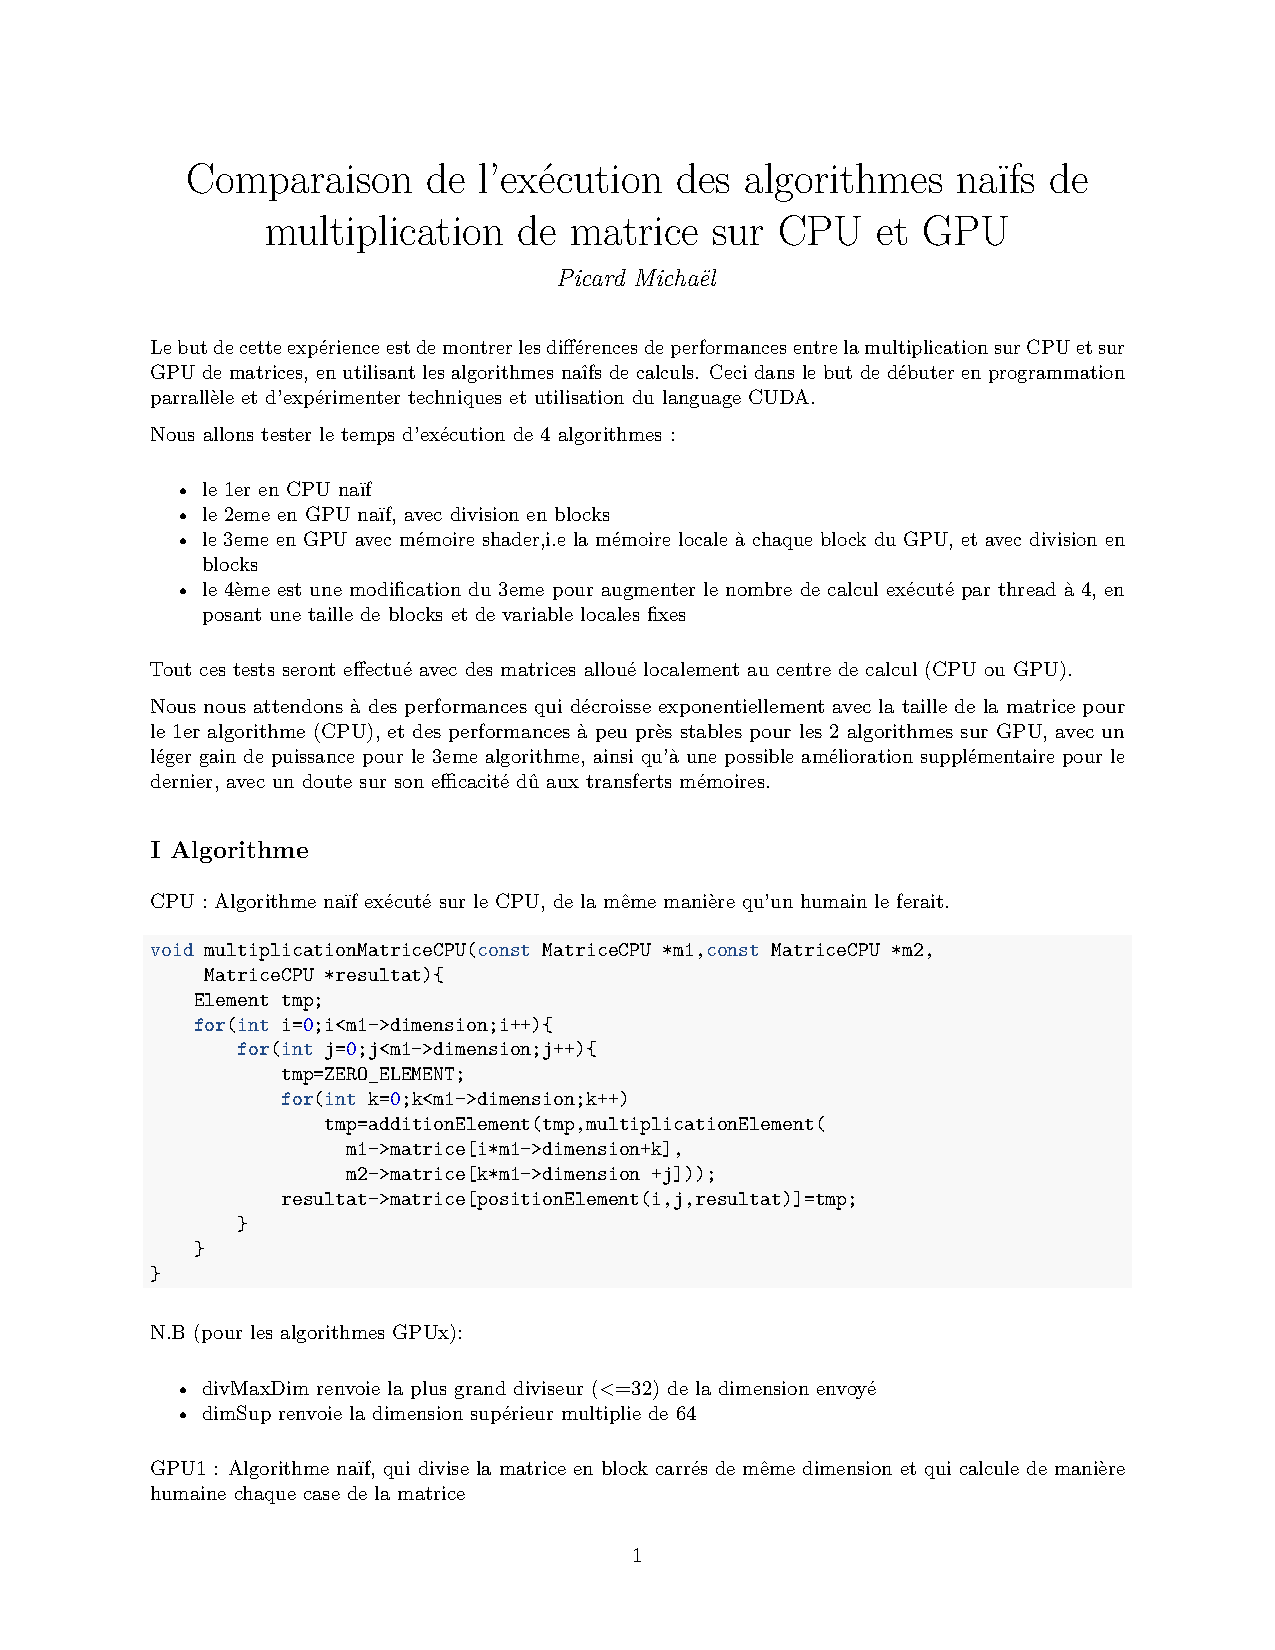
\includepdf[pages=-]{analyse.pdf}
\end{document}